\section{Конструкторский раздел \hfill}
\vspace{\baselineskip}

В данном разделе представлены последовательный и параллельный алгоритмы численного интегрирования методом средних прямоугольников и методом трапеций.

\subsection{Разработка алгоритмов}

На рисунках \ref{fig:diagram-calc-int}-\ref{fig:diagram-int-trapez} представлены схемы последовательных алгоритмов численного интегрирования, на рисунках \ref{fig:diagram-calc-int-par}-\ref{fig:diagram-int-trapez-par} -- схемы параллельных алгоритмов.

\begin{figure}[h!btp]
	\centering
	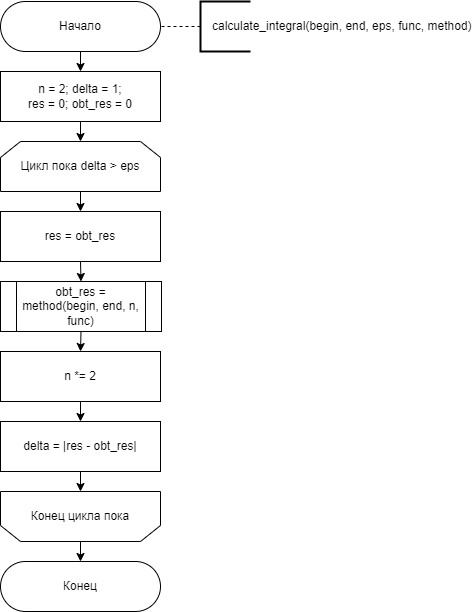
\includegraphics[width=280pt]{inc/calc_int.png}
	\caption{Схема последовательного алгоритма численного интегрирования с заданной точностью}
	\label{fig:diagram-calc-int}	
\end{figure}

\clearpage

\begin{figure}[h!btp]
	\centering
	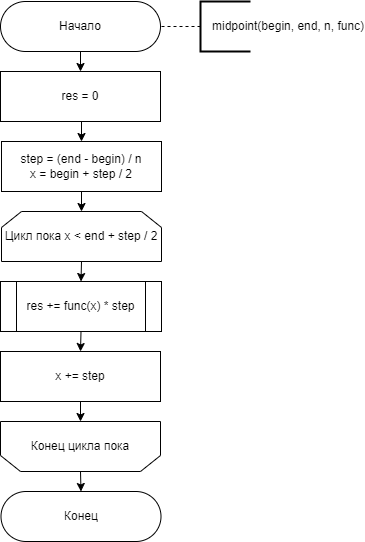
\includegraphics[width=190pt]{inc/int_midpoint.png}
	\caption{Схема последовательного алгоритма численного интегрирования методом средних прямоугольников при заданном $n$}
	\label{fig:diagram-int-midpoint}	
\end{figure}

\begin{figure}[h!btp]
	\centering
	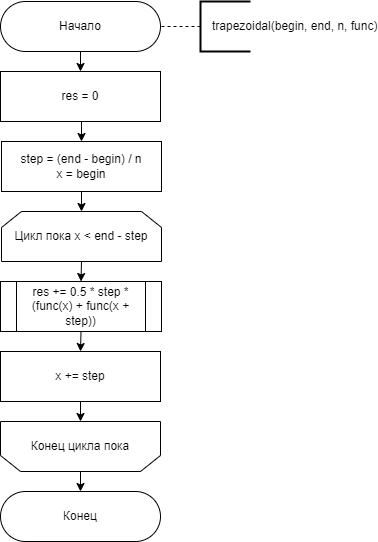
\includegraphics[width=190pt]{inc/int_trapez.png}
	\caption{Схема последовательного алгоритма численного интегрирования методом трапеций при заданном $n$}
	\label{fig:diagram-int-trapez}	
\end{figure}

\clearpage

\begin{figure}[h!btp]
	\centering
	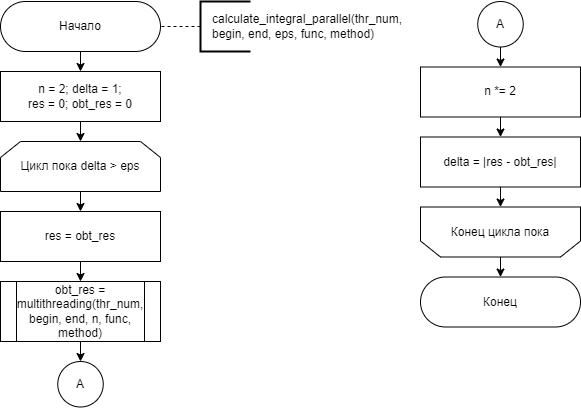
\includegraphics[width=300pt]{inc/calc_int_par.png}
	\caption{Схема параллельного алгоритма численного интегрирования с заданной точностью}
	\label{fig:diagram-calc-int-par}	
\end{figure}

\begin{figure}[h!btp]
	\centering
	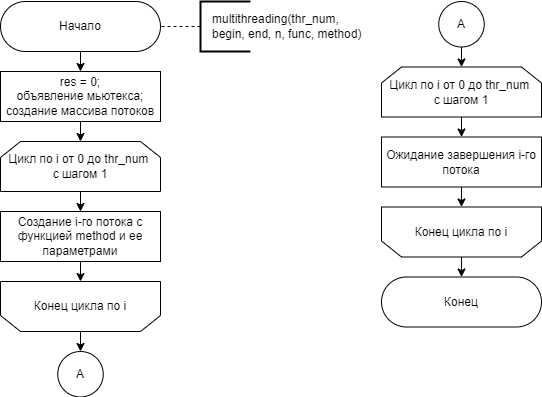
\includegraphics[width=300pt]{inc/multithreading.png}
	\caption{Схема создания потоков для параллельного алгоритма численного интегрирования}
	\label{fig:diagram-multithreading}	
\end{figure}

\clearpage

\begin{figure}[h!btp]
	\centering
	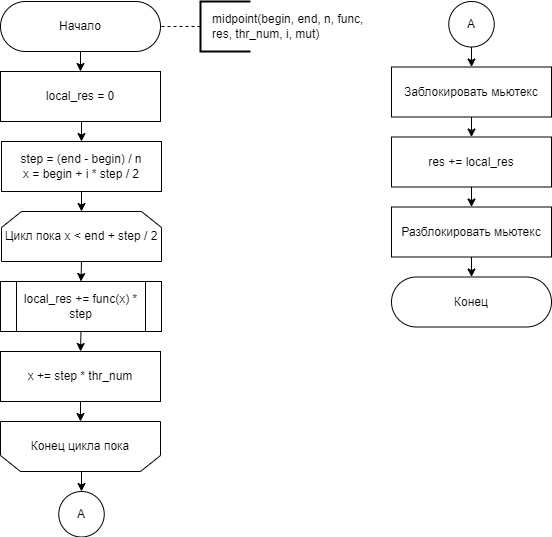
\includegraphics[width=250pt]{inc/int_midpoint_par.png}
	\caption{Схема параллельного алгоритма численного интегрирования методом средних прямоугольников при заданных $n$ и номере потока}
	\label{fig:diagram-int-midpoint-par}	
\end{figure}

\begin{figure}[h!btp]
	\centering
	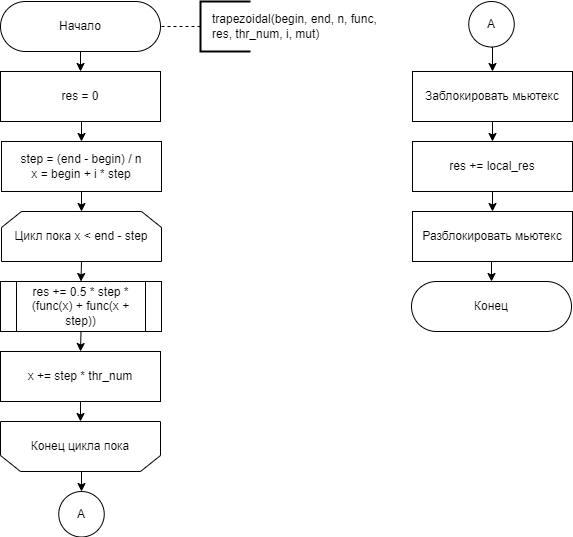
\includegraphics[width=250pt]{inc/int_trapez_par.png}
	\caption{Схема параллельного алгоритма численного интегрирования методом трапеций при заданных $n$ и номере потока}
	\label{fig:diagram-int-trapez-par}	
\end{figure}

\subsection*{Вывод}

Были разработаны схемы последовательного и параллельного алгоритмов численного интегрирования.
